\chapter{Estimating the luminosity}
%\epigraph{salimmo sù, el primo e io secondo, \\
%tanto ch’i’ vidi de le cose belle \\
%che porta ’l ciel, per un pertugio tondo.\\ 

%E quindi uscimmo a riveder le stelle.}{Dante, \textit{Inferno XXXIV}}
\epigraph{As for their appearance, the four of them looked alike; each was like a wheel intersecting a wheel. Their entire bodies, including their backs, their hands and their wings, were completely full of eyes, as were their four wheels.}{Ezekiel,10:10-12}
\section{Concept of luminosity}
In particle physics experiments, the energy available for producing new effects is a crucial parameter. This energy is determined by the centre of mass energy, which can be optimized through colliding beams, minimizing energy loss in the motion of the centre of mass system. Another critical aspect is the number of useful interactions or events, especially when studying rare events with a small production cross-section $\sigma_p$. The ability of a particle accelerator to produce the required number of interactions is quantified by the concept of luminosity, defined as the proportionality factor between the number of events per second $\tfrac{dR}{dt}$ and the cross-section. The relation between luminosity $\mathcal{L}$, cross-section $\sigma_p$ and ratio $\tfrac{dR}{dt}$ is defined as:
\begin{equation}
    \frac{dR}{dt} = \mathcal{L}{\sigma_p}\label{lumi_def}
\end{equation}
The unit of luminosity is therefore $\SI{}{\per\centi\meter\squared\per\second}$

Equation \ref{lumi_def} can be used to indirectly estimate luminosity from a known cross section. The basic relationship between luminosity and cross section is given by:

\begin{equation}
\mu_{\text{vis}} = \frac{R_{\text{vis}}}{f} = \frac{L_{\text{inst}} \sigma_{\text{vis}}}{f}\label{mu_def}
\end{equation}

where:
\begin{itemize}
\item  $R_{\text{vis}}$ is the interaction rate of a visible process,
\item  $f$ is the frequency of collisions,
\item  $\mathcal{L}$ is the instantaneous luminosity,
\item  $\sigma_{\text{vis}}$ is the cross section of the chosen visible process, and
\item  $\mu_{\text{vis}}$ represents the average number of visible proton-proton (pp) interactions per crossing.
\end{itemize}
This relationship can be used to measure luminosity indirectly by determining \(\mu_{\text{vis}}\) from effective processes, such as those producing at least two reconstructed VELO tracks. Once \(\mu_{\text{vis}}\) is measured, the luminosity can be derived as follows:

\begin{equation}
\mathcal{L} = \frac{\mu_{\text{vis}} \cdot f}{\sigma_{\text{vis}}}
\end{equation}

This approach is referred to as "relative luminosity determination" because it relies on a known cross section to "calibrate" the luminosity, using it as a normalization factor. During periods of data-taking at LHCb, different "luminosity counters" record the values of visible interactions, allowing researchers to calculate \(\mu_{\text{vis}}\). This data is then used to estimate the instantaneous luminosity, enabling accurate cross-section measurements and experimental calibration.


% Integrated Luminosity Definition
The maximum luminosity, and therefore the instantaneous number of interactions per second, is a significant factor in particle collider experiments. However, the final figure of merit is the integrated luminosity, denoted by $\mathcal{L}_{\text{int}}$. Over a given time period \(T\), it is defined as follows:

\begin{equation}
\mathcal{L}_{\text{int}} = \int_0^T L(t) dt .
\end{equation}
Integrated luminosity is crucial because it directly relates with the total number of events of interest, as indicated by the following expression:

\begin{equation}
\mathcal{L}_{\text{int}} \times \sigma_p = \text{number of events of interest}.
\end{equation}

The unit of integrated luminosity is therefore $\SI{}{\per\centi\meter\squared}$, but more often the barn unit is used, which is defined as $\SI{1}{\barn}=\SI{1e-24}{\per\centi\meter\squared}$. The integrated luminosity is therefore the statistics used for indicated the quantity of data available for the analysis.

% Luminosity Decay Model
A key factor influencing integrated luminosity is the decay of instantaneous luminosity over time, caused by various factors like beam intensity reduction, transverse emittance growth, and bunch length increase. A common model to represent this decay assumes an exponential form:

\begin{equation}
\mathcal{L}(t) = \mathcal{L}_0 \exp\left( -\frac{t}{\tau} \right)
\end{equation}

where $\mathcal{L}_0$ is the initial luminosity, \(t\) is the elapsed time, and \(\tau\) is the lifetime associated with the decay. 

In the following subsection a theoretical description of the instantaneous luminosity concept will be given.
In the next section, I will describe the luminosity at LHCb and explain how at this experiment we can avoid the exponential decay.

\subsection{Luminosity in Fixed Target Experiments}
In fixed target experiments, the luminosity is influenced by the properties of both the incoming beam and the stationary target. The incoming beam is characterized by its flux $\Phi$, which is the number of particles per second. The target is described by its density $\rho_T$ and its length $l$. The luminosity in this setup is calculated using the formula:

\[
\mathcal{L}_{FT} = \Phi \cdot \rho_T \cdot l
\]

Given this definition, the interaction rate can be expressed as:

\[
\frac{dR}{dt} = \Phi \cdot \rho_T \cdot l \cdot \sigma_p
\]

\subsection{Luminosity in Colliding Beam Experiments}
In colliding beam experiments, both beams act as the target and the incoming beam simultaneously. The general expression for luminosity in this case involves the convolution of the 3-D distribution functions of the beams, considering the overlap integral. A schematic picture is shoen in Figure \ref{fig:lumi-def}\cite{Herr:941318}. Since the two beams are not stationary but moving through each other, the overlap integral depends on the longitudinal position of the bunches and therefore on the time as they move towards and through each other. For our integration we use the distance of the two beams to the central collision point $s_0 = ct$ as the ”time” variable. 
The luminosity is proportional to the overlap integral of the two  $\rho_1$, $\rho_2$ time dependent beam density distribution function:

\begin{figure}
    \centering
    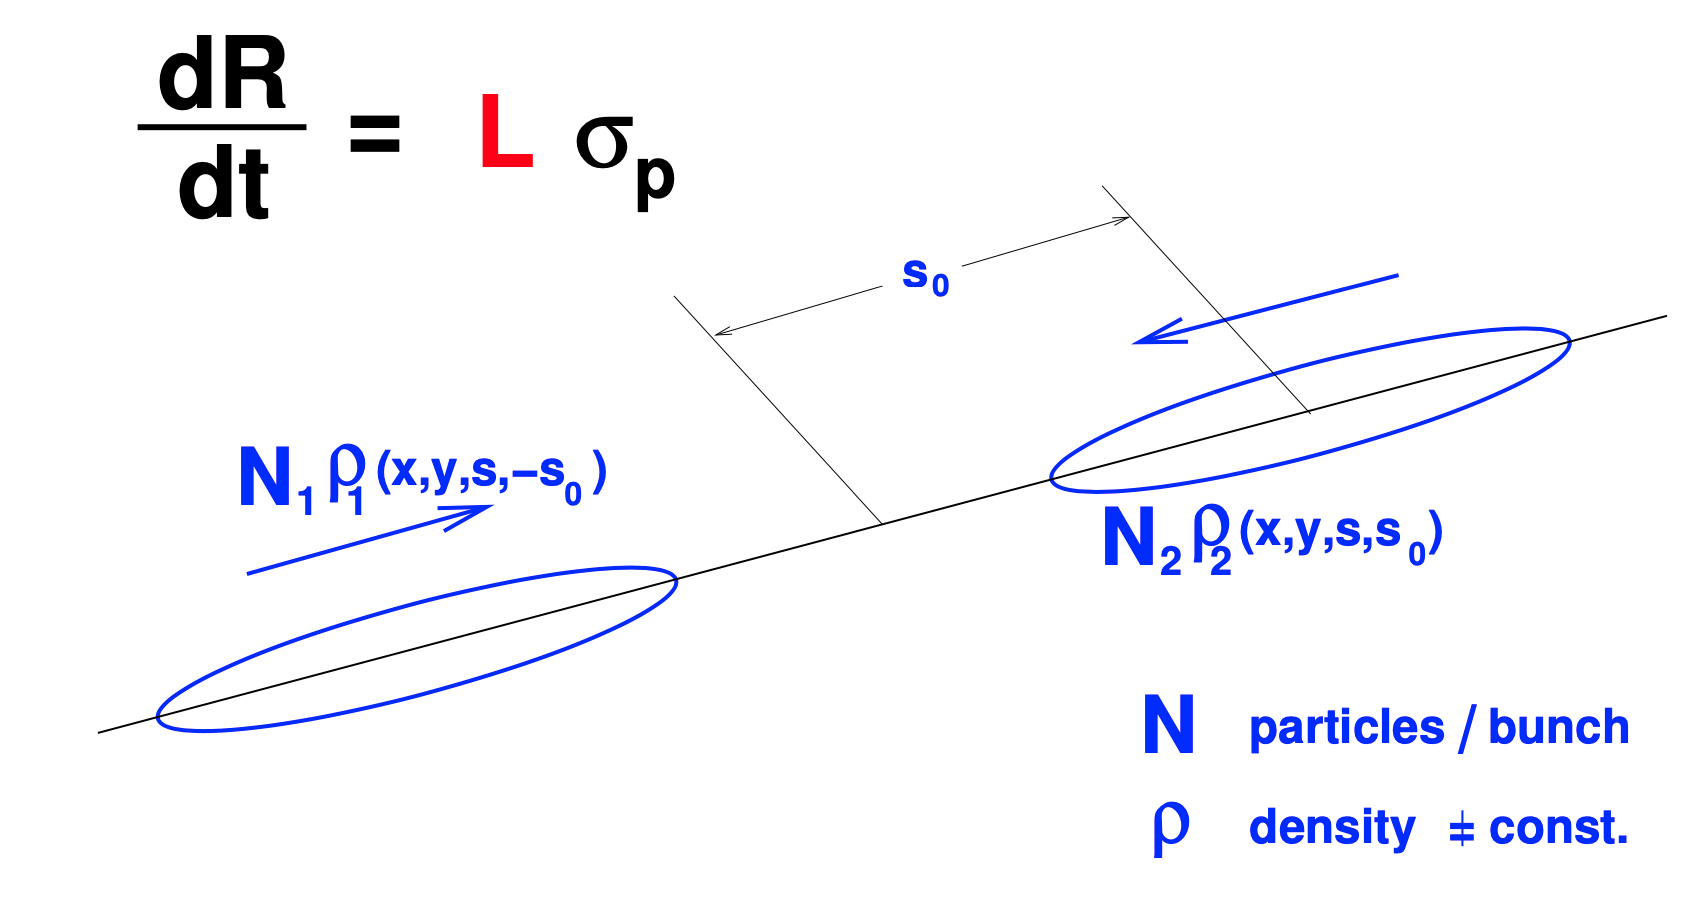
\includegraphics[width=0.6\textwidth]{figures/luminosity_def.png}
    \caption{Schematic view of a colliding beam interaction.}
    \label{fig:lumi-def}
\end{figure}

\begin{equation}
    \mathcal{L} \propto K\cdot\int\int\int\int_{-\infty}^{+\infty}\rho_1(x,y,s,s_0)\rho_2(x,y,s,s_0)dxdydsds_0.
\end{equation}

Assuming colliding bunches moving against each other that meet at $s_0$, we have to take into account the kinematic factor\cite{Moller}:
\begin{equation}
    K = \sqrt{\bigl(\vec{v_1}-\vec{v_2}\bigr)^2-\bigl(\vec{v_1} \times \vec{v_2}\bigr)^2/c^2}.
\end{equation}
By further assuming head-on collisions ($\vec{v_1}=-\vec{v_2}$) and that all densities are uncorrelated in all planes, we can write:
\begin{equation}
        \mathcal{L} = 2 N_1 N_2 f N_b\cdot\int\int\int\int_{\infty}^{+\infty}\rho_{1x}(x)\rho_{1y}(y)\rho_{1s}(s+s_0)\rho_{2x}(x)\rho_{2y}(y)\rho_{2s}(s+s_0)dxdydsds_0.\label{beam_overlap}
\end{equation}

where:
\begin{itemize}
    \item \( N_1 \) and \( N_2 \) are the number of particles per bunch for each beam.
    \item \( f \) is the revolution frequency.
    \item \( N_b \) is the number of bunches in each beam.
\end{itemize}

To evaluate this integral one should know all distributions. An analytical calculation is not always possible and a numerical integration may be required. However in many cases the beams follow ”reasonable” profiles and we can obtain closed solutions. It is often assumed that the beam profiles follow Gaussian distributions. This assumption is justified because the luminosity is determined by the overlap of the core of the distributions, with the tails contributing minimally.
Given Gaussian profiles, we can write the distribution function for a Gaussian beam in a general form:
\begin{equation}
\rho_{iz}(z) =\frac{1}{\sigma_z\sqrt{2\pi}} \exp\left( -\frac{z^2}{2 \sigma_z^2} \right) \text{ where } i=1,2, \quad z=x,y
\end{equation}
\begin{equation}
\rho_{s}(s\pm s_0) =\frac{1}{\sigma_s\sqrt{2\pi}} \exp\left( -\frac{(s\pm s_0)^2}{2 \sigma_s^2} \right)
\end{equation}

Let's assume equal beams, i.e.  $\sigma_{iz} = \sigma_{iz}$ for $i=1,2$, z=$x,y,s$ and that the number of particles per bunch (\( N_1 \) and \( N_2 \)), revolution frequency (\( f \)), and number of bunches (\( N_b \)) are known. For exactly head-on collisions, where the bunches travel nearly at the speed of light, the kinematic factor becomes 2.

Using this information, the integral for luminosity can be derived by first considering the overlap integral of the Gaussian distributions as in equation \eqref{beam_overlap}:

\begin{equation}
\mathcal{L} = \frac{2  N_1 N_2 f N_b}{(\sqrt{2\pi})^6 \sigma_x^2\sigma_y^2\sigma_s^2}\int\int\int\int e^{-\frac{x^2}{2 \sigma_x^2}} e^{-\frac{y^2}{2 \sigma_y^2}} e^{-\frac{s^2}{2 \sigma_s^2}}e^{-\frac{s_0^2}{2 \sigma_s^2}}dxdydsds_0.
\end{equation}

After integrating over $s$ and $s_0$\footnote{Gassuain integral: $\int_{-\infty}^{+\infty}e^{-at^2}dt = \sqrt{\tfrac{\pi}{a}}$}, we git a first intermediate result:
\begin{equation}
    \mathcal{L} = \frac{2  N_1 N_2 f N_b}{8(\sqrt{\pi})^4 \sigma_x^2\sigma_y^2}\int\int \exp\left(-\frac{x^2}{2 \sigma_x^2}\right) \exp\left(-\frac{y^2}{2 \sigma_y^2}\right) dxdy .
\end{equation}

Finally, after integration over x and y, we get the well-known formula of luminosity for colliding Gaussian beams with head-on collisions:

\begin{equation}
\mathcal{L} = \frac{N_1  N_2  f N_b}{4 \pi  \sigma_x \sigma_y}.
\end{equation}

If we generalize to the case where the x and y beam profiles are unequal but still assume approximately equal bunch lengths (\( \sigma_{1s} \approx \sigma_{2s} \)), we get a modified formula for luminosity:

\begin{equation}
\mathcal{L} = \frac{N_1  N_2  f  N_b}{2 \pi \sqrt{(\sigma_{1x}^2 + \sigma_{2x}^2)(\sigma_{1y}^2 + \sigma_{2y}^2)}}.
\end{equation}

\subsection{Effect of crossing angles and beam displacement}
When beams do not collide head-on but with a small transverse offset, or if they cross at an angle, modifications to the standard luminosity calculation are required. These changes arise from differences in the spatial distribution of the beams during collision. In this section, we derive the luminosity for cases with crossing angles and offsets, leading to a more general formula.

\begin{figure}
    \centering
    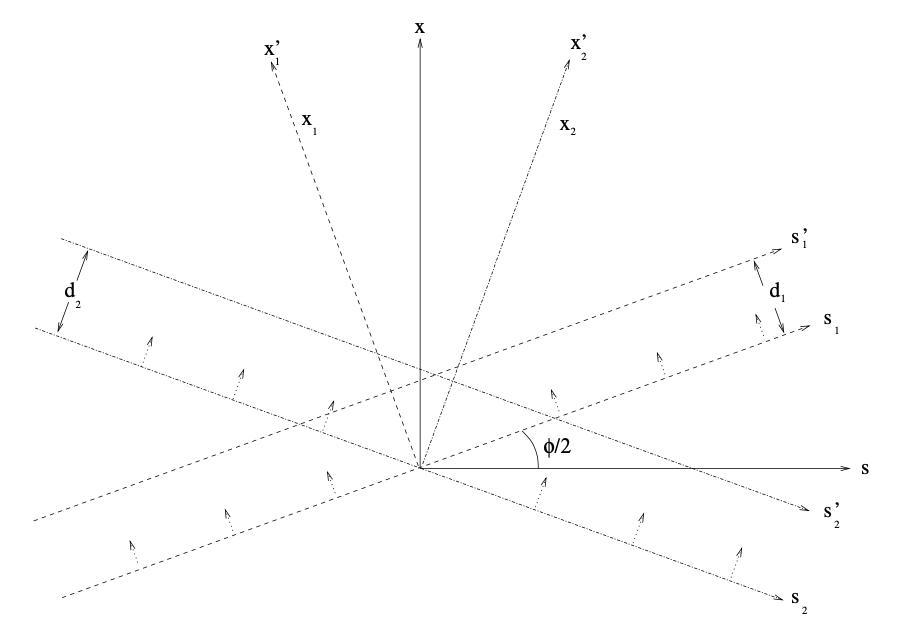
\includegraphics[width=0.7\textwidth]{figures/lumi_geometry.png}
    \caption{Schematic view of two bunches colliding at a finite crossing angle and an offset between the two beams with respect to the reference xs}
    \label{fig:lumi-geometry}
\end{figure}

Consider a scenario where two beams do not collide head-on but cross with an angle and have transverse offsets. The modified geometry is shown in Figure \ref{fig:lumi-geometry}, where beam 1 is displaced by \(d_1\) and beam 2 by \(d_2\) with respect to their reference orbits. The following coordinate transformations are applied:

\begin{equation}
\begin{aligned}[t]
x_1 &= d_1 + x \cos(\phi),  \\
s_1 &= s \cos(\varphi) - x \sin(\varphi),
\end{aligned}
\qquad
\begin{aligned}[t]
       x_2 &= d_2 + x \cos(\varphi), \\
        s_2 &= s \cos(\varphi) + x \sin(\varphi).
\end{aligned}
\end{equation}

Using these transformations, we calculate the luminosity for this modified setup. Following similar integration strategies and approximations as before, but taking into account the coordinate transformations, we can derive the luminosity for this scenario.

After integrating over the \(y\) and \(s_0\) coordinates, the luminosity formula for beams with crossing angles and transverse offsets becomes:

\begin{align}
\mathcal{L} = \frac{N_1 N_2  f  N_b}{8 \pi^2  \sigma_x^2 \sigma_y  \sigma_s} 2 \cos^2\frac{\varphi} {2}\int\int &e^{-\frac{x^2 \cos^2(\varphi/2) + s^2 \sin^2(\varphi/2)}{2 \sigma_x^2}}e^{-\frac{x^2 \sin^2(\varphi/2) + s^2 \cos^2(\varphi/2)}{2 \sigma_x^2}}\\
\times & e^{-\frac{d_1^2+d_2^2+2(d_1+d_2)x\cos(\varphi/2)-2(d_2-d_1)s\sin(\varphi/2)}{2\sigma_x^2}}dxds.
\end{align}

Integrating over \(x\)\footnote{eccxtended gaussian integral: $\int_{-\infty}^{+\infty}e^{-(at^2+bt+c)}dt = \sqrt{\pi/a}e^{\frac{b^2-ac}{a}}$}, the resulting expression for luminosity, including the effects of crossing angles and offsets, is:

\begin{equation}
\mathcal{L} = \frac{N_1 \cdot N_2 \cdot f \cdot N_b}{8 \pi^2 \sigma_s} 2\cos\frac{\varphi}{2} \int_{-\infty}^{+\infty}W \frac{e^{-As^2 + 2Bs}}{\sigma_x\sigma_y}ds,
\end{equation}

where \(A\) and \(B\) are defined as follows:

\begin{equation}
A = \frac{\sin^2\frac{\varphi}{2}}{\sigma_x^2} + \frac{\cos^2\frac{\varphi}{2}}{\sigma_s^2} \frac{d_2 - d_1}{2 \sigma_x^2}, \quad
B = \frac{(d_2 - d_1)\sin(\varphi/2)}{2 \sigma_x^2}.
\end{equation}

and 

\begin{equation}
    W = e^{-\frac{1}{4\sigma_x^2}(d_2-d_1)^2}
\end{equation}

With these definitions, the factorization of the luminosity formula becomes straightforward. The following correction factors emerge:
\begin{itemize}
\item $W$ accounts for the presence of beam offsets.
\item $e^{B^2/A}$ represents the reduction due to crossing angles and offsets.
\item $S$ is a calculated luminosity reduction factor for crossing angles alone, defined as:
\end{itemize}

\begin{equation}
  S = \frac{1}{\sqrt{1 + \left( \frac{\sigma_s}{\sigma_x} \tan \frac{\varphi}{2} \right)^2}} \approx \frac{1}{\sqrt{1 + \left( \frac{\sigma_s}{\sigma_x} \frac{\varphi}{2} \right)^2}}
\end{equation}

which can be interpreted as a correction to the beam size, thus introducing an ``effective beam size":
\begin{equation}
    \sigma_{eff} = \sigma \sqrt{1+\biggl(\frac{\sigma_s}{\sigma_x}\frac{\varphi}{2}\biggr)^2}.
\end{equation}

Thus, the final expression for luminosity in the presence of crossing angles and beam offsets is:

\begin{equation}
\mathcal{L} = \frac{N_1  N_2  f  N_b}{4 \pi  \sigma_x  \sigma_y} \cdot W \cdot e^{B^2/A} \cdot S.
\end{equation}

\section{An absolute luminosity calibration: The Van Der Meer scan}
\textit{Explaination of what VdM is and how we use it to calibrate luminosity.}\\
Van der Meer scan luminosity measurement and beam–beam correction, Vladislav Balagura



\section{Luminosity at LHCb}
In late 2009, LHCb recorded its first proton-proton (pp) collisions at an injection energy of $\sqrt{s}=\SI{0.9}{\tera\eV}$. These data were used to finalize the commissioning of the sub-detector systems, calibration, and the alignment of tracking, calorimeter, and particle identification (PID) systems. During this period, the VELO was left in the open position to accommodate the larger aperture required at lower beam energies.
The operating conditions changed rapidly in 2010 due to the LHC ramp-up in luminosity. A critical parameter for LHCb performance is the pile-up \(\mu_{\text{vis}}\), defined in Eq. \ref{mu_def} as the average number of visible interactions per beam-beam crossing. Luminosities started around $\sim \SI{1e28}{\per\centi\meter\squared\per\second}$ with almost no pile-up but eventually reached $\sim \SI{1e32}{\per\centi\meter\squared\per\second}$ with $\mu_{\text{vis}} \approx 2.5$.
While the highest luminosity in 2010 was already 75\% of the LHCb design luminosity, the pile-up was much larger due to the low number of bunches in the machine. Despite this, the trigger and reconstruction systems demonstrated efficient performance under these conditions\cite{det_perf}.

\begin{figure}
    \centering
    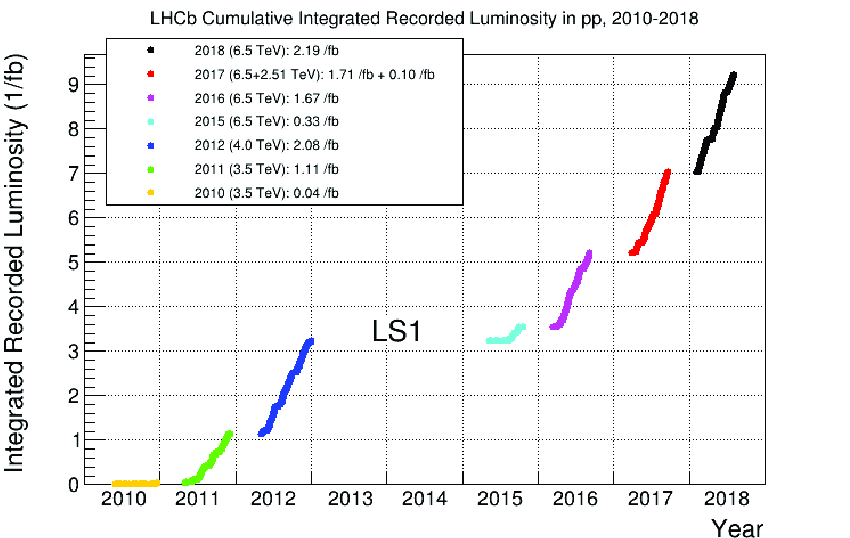
\includegraphics[width=\textwidth]{figures/lumiRun2.png}
    \caption{Integrated luminosity during Run1 and Run2, interspersed by the LS1.}
    \label{fig:lumiRun1Run2}
\end{figure}

The LHC beam energy was 3.5 TeV during 2010 and 2011. In 2011, the number of bunches in the machine increased to about 1300, allowing for a reduction in pile-up while LHCb operated at a luminosity of $\SI{3.5e32}{\per\centi\meter\squared\per\second}$. This was 1.75 times the design luminosity of $\sim \SI{2e32}{\per\centi\meter\squared\per\second}$. The instantaneous luminosity directly delivered by the LHC was too high with respect to the target luminosity the LHCb experiment has been designed for, since of the too high event rate and irradiation dose to which the detectors would be subjected. Since of the higher detector hits multiplicity, track and vertex reconstructions would suffer of high event pile-up, that increases combinatorial background and complicates track reconstruction.
To cope with this issue, in 2011 the LHCb experiment introduced a luminosity levelling procedure at the LHCb interaction point to keep the instantaneous luminosity stable within about 5\% during a fill. This was achieved by adjusting the transverse overlap of the beams. For one particularly long fill, a maximum overlap with head-on beams was reached only after 15 hours. This levelling minimized the effects of luminosity decay and allowed LHCb to maintain a consistent trigger configuration, reducing systematic uncertainties due to changing detector occupancy.

In 2012, the LHC beam energy was increased to $\SI{4}{\tera\eV}$, and LHCb took data at a luminosity of $\sim \SI{4e32}{\per\centi\meter\squared\per\second}$, twice the LHCb design luminosity. An effort was made in 2012 to use more efficiently the processing power available in the Event-Filter-Farm (EFF) in order to cope with the increase in luminosity, allowing LHCb to increase the data sample available for physics analysis. This value of luminosity was kept as target until the end of Run2. 


For Run3, LHCb plan to further increase this value by 5, reaching an instantaneous luminosity of $\SI{2e33}{\per\centi\meter\squared\per\second}$
An overview of the luminosity integrated until the end of Run 2 is depicted in Figure \ref{fig:lumiRun1Run2}.

\subsection{Luminosity leveling}

\begin{figure}
    \centering
    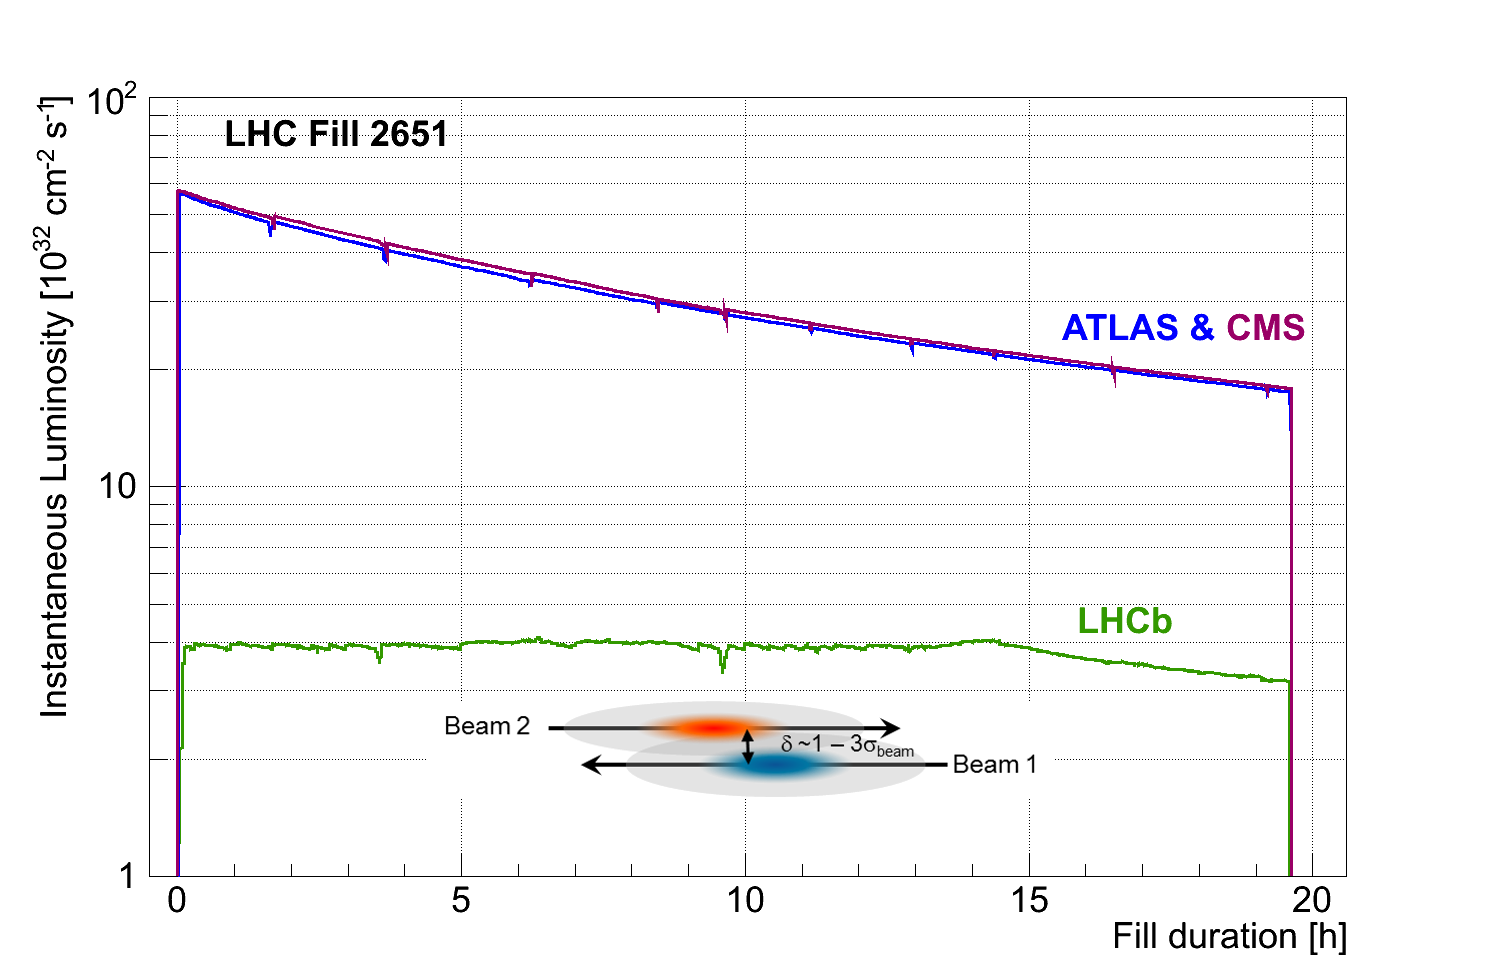
\includegraphics[width=\textwidth]{figures/luminosity_leveling.png}
    \caption{Development of the instantaneous luminosity for ATLAS, CMS and LHCb during LHC fill 2651. After ramping to the desired value of $\SI{4e32}{\per\centi\meter\squared\per\second}$ for LHCb, the luminosity is kept stable in a range of 5\% for about 15 hours by adjusting the transversal beam overlap.
    The difference in luminosity towards the end of the fill between ATLAS, CMS and LHCb is due to the difference in the final focusing at the collision points, commonly referred to as the beta function $\beta*$}
    \label{fig:lumi-leveling}
\end{figure}

Luminosity levelling is a critical technique used by the LHCb experiment to stabilize the instantaneous luminosity and control pile-up at the experiment's interaction point. It addresses the issue of excessively high event rates and irradiation doses caused by the high luminosity delivered by the LHC, which can complicate track reconstruction and increase systematic uncertainties.
The instantaneous luminosity in the LHCb experiment is kept constant at a lower value compared to other LHC experiments like CMS and ATLAS. Generally, the luminosity in an LHC fill follows an exponential decay trend due to beam intensity degradation effects. However, by using luminosity levelling, LHCb maintains the luminosity at a fixed peak value, allowing for consistent operational conditions for the DAQ and trigger systems.  This behaviour is well depicted in Figure \ref{fig:lumi-leveling}. Precision in the online measurement of instantaneous luminosity is vital for monitoring and luminosity levelling. The collaboration has estimated that an accuracy of less than 5\% is sufficient for this purpose. 


Luminosity levelling is achieved by adjusting the transverse overlap between the two colliding beams using corrector magnets located on each side of the experiment. The beam overlap is incrementally increased in small discrete steps as the beam intensity decreases, allowing for fine control of the luminosity. The adjustments are made through a luminosity control software, which provides feedback from the LHCb sub-detectors to the LHC Control Centre. A scheme of this software is reported in Figure \ref{fig:lumi-control}.
The LHCb luminosity control manager, part of the ECS, is a FSM driven by LHC operational modes. It monitors the instantaneous luminosity, compares it to the optimal target luminosity, and sends the levelling parameters to the LHC Lumi Levelling driver application. On the LHC side, this application uses a ``levelling algorithm" to determine the necessary adjustments in beam separation to maintain the target luminosity.

\begin{figure}
    \centering
    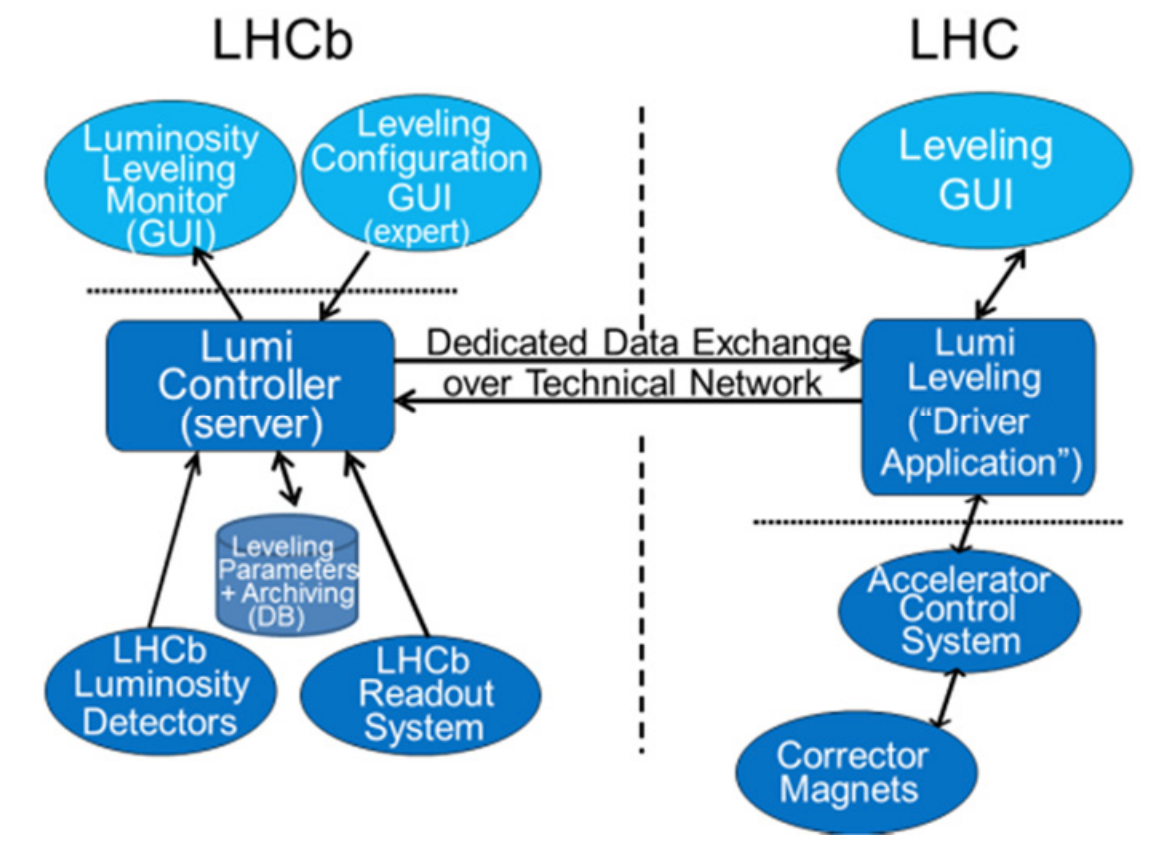
\includegraphics[width=0.8\textwidth]{figures/lumi_control.png}
    \caption{LHCb Luminosity control software diagram}
    \label{fig:lumi-control}
\end{figure}

\subsection{Luminometers}
The target luminosity for LHCb is a compromise between physics priorities, trigger selection efficiencies, detector performance limitations, DAQ system constraints, and offline data-processing capabilities. For Run-2, this value was set to $\SI{4e32}{\per\centi\meter\squared\per\second}$, while for Run-3, the optimal target luminosity is estimated at $\SI{2e33}{\per\centi\meter\squared\per\second}$, corresponding to a pile-up per bunch-crossing of approximately $\mu = 5.5$.

During Run-1 and Run-2, online luminosity estimates had a precision of 10\% and were derived from two primary sources: 
\begin{enumerate}
    \item Transverse Energy Deposition: Observations of energy depositions over a fixed threshold in the calorimeter system;
    \item Muon Station Counts: Counts in the muon stations, provided by the Level-0 (L0) hardware-trigger.
\end{enumerate}
\paragraph{PLUME}
A dedicated luminometer sub-detector, PLUME (Probe for LUminosity MEasurement), was introduced for Run-3 to improve both online and offline luminosity measurement precision. PLUME consists of 24 hodoscopes (couples of detector modules read out for coincidences in both modules) surrounding the beampipe, pointing at the nominal interaction point, and located approximately 1.7 meters upstream from the collision region. It covers a high-pseudorapidity range $(2.4 < \eta < 3.1)$.

Each hodoscope module is composed of 10 × 10 × \SI{5}{\milli\meter\tothe{3}} quartz crystals, coupled with photomultipliers that detect Cherenkov light generated when high-speed particles traverse the quartz. Online luminosity measurement is performed by counting coincidences in at least one hodoscope, identifying tracks coming from the interaction region, and suppressing background activity.
In addition to the PLUME detector, LHCb introduced several other luminosity counters for online monitoring and offline luminosity measurement. This redundancy provides stability cross-checks and helps evaluate systematic uncertainties.

A problem with the luminosity linearity has been discovered in September 2022: due to non-negligible rate of random coincidences the PLUME showed divergencies from the expected linear behaviour. Since 7th of July 2022 PLUME luminosity corrected for non-linearity using HLT1 counters, rendering de-facto PLUME an offline luminosity estimator.

DA AGGIUNGERE QUALCOSA SULLA NON LINEARITÀ DI PLUME?

\paragraph{Other online counters} 
In addition to PLUME, there are other counters based on minimum bias conditions and independent of high-level reconstruction sequences, operating at approximately 30 MHz and read out via the ECS interface. These counters are primarily used for online monitoring and include:
\begin{itemize}
   \item VELO clusters counters based on FPGA (object of this thesis)
   \item VELO superpixel ASICS counters
   \item RICH currents counters
   \item SciFi currents counters
\end{itemize}
\paragraph{Offline counters} 
Other than online counters, there are also implemented offline counters for more precise estimates.
These counters are based on the number of reconstructed tracks, primary vertices, hits or energy deposited\
We distinguish between HLT1 (processed at ∼30 kHz) and HLT2 counters (offline).

The HLT1 counters include:
\begin{itemize}
   \item Number of muon hits in the muon stations (luMUONmeter).
   \item  VELO tracks in bins of $\eta$ and reconstructed primary vertices.
   \item SciFi clusters per module combinations.
   \item Energy deposition in the ECal and HCal.
\end{itemize}
The HLT2 counters are:
\begin{itemize}
    \item Hits in the RICH1 and RICH2 detectors.
    \item calorimeters counters after zero suppression 
\end{itemize}

\section{Online VELO Luminosity counters}

\section{Combining the counters for a single luminosity measurement}
\textit{How we combine the 208 available measurements of luminosity: study on which estimator to choose between mean, median and trimmed mean}